\section*{Assignment 03: Evolution of the Platform Concept}
\addcontentsline{toc}{section}{Assignment 03: Evolution of the Platform Concept}

\subsection*{Where we started}
Our first sketches revolved around a ``dinner experiences'' marketplace that matched home chefs with curious guests. It fit the zeitgeist but clashed with why we joined the course. Early interviews and the VirtuAI quick-case debrief \citep{Gunasilan2024} exposed two red flags: regulators already scrutinise informal food businesses, and we had zero logistics advantage. Overlaying \citet{Choudary2016}'s typology made it obvious we were drifting toward an asset-heavy service, not the orchestrator we wanted to study.

\subsection*{Moments that changed the trajectory}
The pivotal moment came during Session~6 when a guest NGO described how hard it is to scope student projects without hand-holding. That story made us revisit our own campus experience and birthed SkillSync: a student--organisation matchmaking platform focused on scoped, time-bound collaborations. We mapped the new interaction using the platform design toolkit from \citet{Reillier2017}, prototyped scoping templates in Figma, and ran hallway tests with five NGOs from previous course projects. Another turning point was analysing monetisation for the home-chef idea. The numbers crumbled under \citet{Porter2008}'s competitive pressure, yet the same analytical exercise illuminated how SkillSync could monetise through completion-based fees and partner enablement. The pivot looked dramatic on paper, but in practice it was a sequence of incremental bets guided by data and theory, echoing the cautionary tales from Lecture~6 about platforms that misread winner-take-all dynamics \citep{Lecture06}.

\subsection*{Reflection on the path taken}
Was sticking with SkillSync the optimal play? Mostly yes. The concept matches our comparative advantage (campus networks plus student-consulting experience) and gives us a clean cross-side interaction to analyse. We did move too slowly on validating willingness to pay. If I could rewind, I would run pricing conversations alongside prototyping instead of waiting for a polished deck---\citet{HagiuWright2013} warn that deferring business-model validation makes pivots harder later---and I would keep a thinner backlog so sunk-cost bias pops sooner.

Figure~\ref{fig:project-creation} grounds the pivot. The organisation-side wizard forces clarity on outcomes, timelines, support assets, and evaluation criteria, with helper text so NGOs feel coached rather than interrogated. A progress bar sets expectations, and during testing a volunteer coordinator realised she could reuse survey questions as project milestones---a small proof the pivot had legs.

\begin{figure}[h]
  \centering
  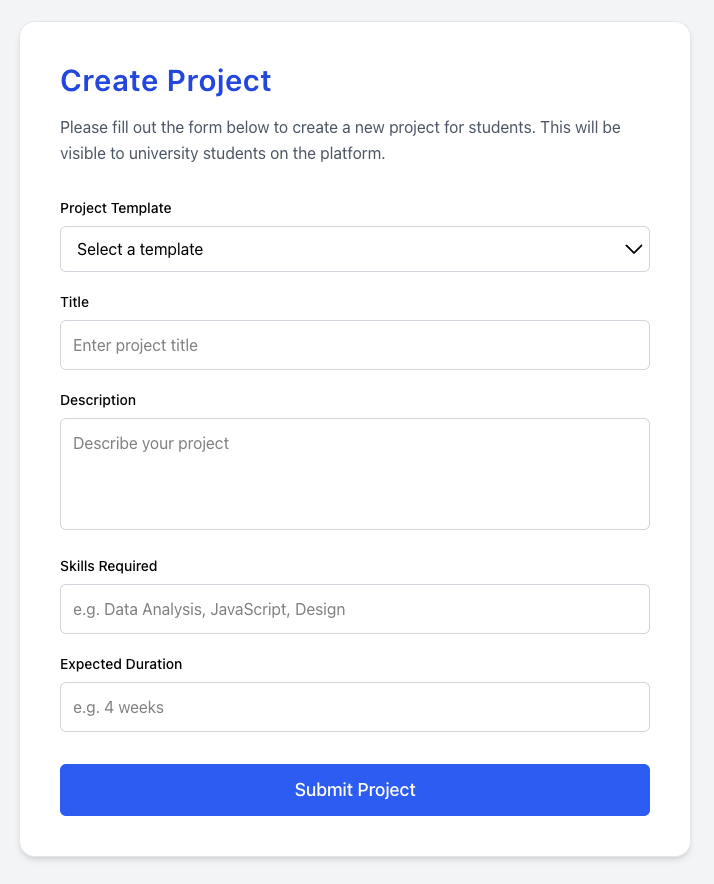
\includegraphics[width=0.7\linewidth]{figures/Organisation-generate-project.png}
  \caption{Organisation project creation wizard (`Organisation-generate-project.png`) designed after the SkillSync pivot.}
  \label{fig:project-creation}
\end{figure}

The expanded scope also let us document decision hygiene. Fortnightly retros scored each experiment on desirability, feasibility, and viability. When the food marketplace kept ranking low on feasibility (licensing, hygiene, logistics) the notes gave us confidence to pivot despite sunk costs, while SkillSync experiments scored high on desirability and acceptable on feasibility thanks to campus networks. Documenting those rituals shows how we operationalised \citet{Choudary2016}'s iterative governance and \citet{Srnicek2017}'s legitimacy checks.
